%
% This document contains the chapter about other transmission lines.
%
% Copyright (C) 2006, 2007, 2009 Stefan Jahn <stefan@lkcc.org>
%
% Permission is granted to copy, distribute and/or modify this document
% under the terms of the GNU Free Documentation License, Version 1.1
% or any later version published by the Free Software Foundation.
%

\chapter{Other types of transmission lines}
%\addcontentsline{toc}{chapter}{Other types of transmission lines}

\section{Coaxial cable}
%\addcontentsline{toc}{section}{Coaxial cable}

\begin{figure}[ht]
\begin{center}
\psfrag{er}{$\mathrm{\varepsilon_r}$}
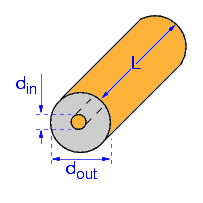
\includegraphics[width=0.35\linewidth]{coax}
\end{center}
\caption{coaxial line}
\label{fig:coax}
\end{figure}
\FloatBarrier

\subsection{Characteristic impedance}
%\addcontentsline{toc}{subsection}{Characteristic impedance}

The characteristic impedance of a coaxial line can be calculated as follows:
\begin{equation}
Z_L = \dfrac{Z_{F0}}{2\pi\cdot\sqrt{\varepsilon_r}}\cdot\ln{\left(\dfrac{D}{d}\right)}
\end{equation}

\subsection{Losses}
%\addcontentsline{toc}{subsection}{Losses}

Overall losses in a coaxial cable consist of dielectric and conductor
losses.  The dielectric losses compute as follows:
\begin{equation}
\alpha_d = \dfrac{\pi}{c_0}\cdot f\cdot \sqrt{\varepsilon_r} \cdot \tan{\delta}
\end{equation}

The conductor (i.e. ohmic) losses are specified by
\begin{equation}
\alpha_c = \dfrac{1}{2}\cdot \sqrt{\varepsilon_r} \cdot\left(\dfrac{\dfrac{1}{D} + \dfrac{1}{d}}{\ln{\left(\dfrac{D}{d}\right)}}\right)\cdot\dfrac{R_S}{Z_{F0}}
\end{equation}

with $R_S$ denoting the sheet resistance of the conductor material,
i.e. the skin resistance
\begin{equation}
R_S = \sqrt{\pi\cdot f\cdot \mu_r \cdot \mu_o \cdot \rho}
\end{equation}

\subsection{Cutoff frequencies}
%\addcontentsline{toc}{subsection}{Cutoff frequencies}

In normal operation a signal wave passes through the coaxial line as a
TEM wave with no electrical or magnetic field component in the
direction of propagation.  Beyond a certain cutoff frequency
additional (unwanted) higher order modes are excited.
\begin{align}
f_{TE} &\approx \dfrac{2\cdot c_0}{\pi\cdot\left(D + d\right)\cdot\sqrt{\varepsilon_r}}
\;\;\;\;\rightarrow\;\;\;\; \textrm{TE(1,1) mode}\\
f_{TM} &\approx \dfrac{c_0}{\left(D - d\right)\cdot\sqrt{\varepsilon_r}}
\;\;\;\;\rightarrow\;\;\;\; \textrm{TM(n,1) mode}
\end{align}

\section{Twisted pair}
%\addcontentsline{toc}{section}{Twisted pair}

The twisted pair configurations as shown in fig. \ref{fig:twisted}
provides good low frequency shielding.  Undesired signals tend to be
coupled equally into eachline of the pair.  A differential receiver
will therefore completely cancel the interference.

\begin{figure}[ht]
\begin{center}
\psfrag{er}{$\mathrm{\varepsilon_r}$}
\includegraphics[width=0.3\linewidth]{twisted}
\end{center}
\caption{twisted pair configuration}
\label{fig:twisted}
\end{figure}
\FloatBarrier

\subsection{Quasi-static model}

According to P. Lefferson \cite{Lefferson} the characteristic
impedance and effective dielectric constant of a twisted pair can be
calculated as follows.
\begin{align}
Z_L &= \dfrac{Z_{F0}}{\pi\cdot\sqrt{\varepsilon_{r,eff}}}\cdot\textrm{acosh}\left(\dfrac{D}{d}\right)\\
\label{eq:TPereff}
\varepsilon_{r,eff} &= \varepsilon_{r,1} + q\cdot\left(\varepsilon_r - \varepsilon_{r,1}\right)
\end{align}

with
\begin{equation}
\label{eq:TPq}
q = 0.25 + 0.0004\cdot \theta^2
\;\;\;\; \textrm{ and } \;\;\;\;
\theta = \textrm{atan}\left(T\cdot\pi\cdot D\right)
\end{equation}

whereas $\theta$ is the pitch angle of the twist; the angle between
the twisted pair's center line and the twist.  It was found to be
optimal for $\theta$ to be between 20\degree and 45\degree.  $T$
denotes the twists per length.  Eq. \eqref{eq:TPq} is valid for film
insulations, for the softer PTFE material it should be modified as
follows.
\begin{equation}
q = 0.25 + 0.001\cdot \theta^2
\end{equation}

Assuming air as dielectric around the wires yields 1's replacing
$\varepsilon_{r,1}$ in eq. \eqref{eq:TPereff}.  The wire's total
length before twisting in terms of the number of turns $N$ is
\begin{equation}
l = N\cdot\pi\cdot D\cdot\sqrt{1 + \dfrac{1}{\tan^2{\theta}}}
\end{equation}

\subsection{Transmission losses}

The propagation constant $\gamma$ of a general transmission line is
given by
\begin{equation}
\gamma = \sqrt{\left(R' + j\omega L'\right)\cdot \left(G' + j\omega C'\right)}
\end{equation}

Using some transformations of the formula gives an expression with and
without the angular frequency.
\begin{equation}
\label{eq:gamma_rlgc}
\begin{split}
\gamma &= \sqrt{\left(R' + j\omega L'\right)\cdot \left(G' + j\omega C'\right)}\\
&= \sqrt{L'C'}\cdot\sqrt{\dfrac{R'G'}{L'C'} + j\omega\left(\dfrac{R'}{L'} + \dfrac{G'}{C'}\right) - \omega^2}\\
&= \sqrt{L'C'}\cdot\sqrt{\left(\dfrac{1}{2}\cdot\left(\dfrac{R'}{L'} + \dfrac{G'}{C'}\right) + j\omega\right)^2 - \dfrac{1}{4}\cdot\left(\dfrac{R'}{L'} + \dfrac{G'}{C'}\right)^2 + \dfrac{R'G'}{L'C'}}
\end{split}
\end{equation}

For high frequencies eq.{\eqref{eq:gamma_rlgc}} can be approximated to
\begin{equation}
\gamma \approx \sqrt{L'C'}\cdot\left(\dfrac{1}{2}\cdot\left(\dfrac{R'}{L'} + \dfrac{G'}{C'}\right) + j\omega\right)
\end{equation}

Thus the real part of the propagation constant $\gamma$ yields
\begin{equation}
\label{eq:alpha_freq}
\alpha = Re\left\{\gamma\right\} = \sqrt{L'C'}\cdot\dfrac{1}{2}\cdot\left(\dfrac{R'}{L'} + \dfrac{G'}{C'}\right)
\end{equation}

With
\begin{equation}
Z_L = \sqrt{\dfrac{L'}{C'}}
\end{equation}

the expression in eq.\eqref{eq:alpha_freq} can be written as
\begin{equation}
\alpha = \alpha_c + \alpha_d = \dfrac{1}{2}\cdot\left(\dfrac{R'}{Z_L} + G'Z_L\right)
\end{equation}

whereas $\alpha_c$ denotes the conductor losses and $\alpha_d$ the
dielectric losses.

\subsubsection{Conductor losses}

The sheet resistance R' of a transmission line conductor is given by
\begin{equation}
R' = \dfrac{\rho}{A_{eff}}
\end{equation}

whereas $\rho$ is the specific resistance of the conductor material
and $A_{eff}$ the effective area of the conductor perpendicular to the
propagation direction.  At higher frequencies the area of the
conductor is reduced by the skin effect.  The skin depth is given by
\begin{equation}
\delta_s = \sqrt{\dfrac{\rho}{\pi\cdot f\cdot\mu}}
\end{equation}

Thus the effective area of a single round wire yields
\begin{equation}
A_{eff} = \pi\cdot\left(r^2 - (r-\delta_s)^2\right)
\end{equation}

whereas $r$ denotes the radius of the wire.  This means the overall
conductor attenuation constant $\alpha_c$ for a single wire gives
\begin{equation}
\alpha_c = \dfrac{R'}{2\cdot Z_L} = \dfrac{\rho}{2\cdot Z_L\cdot\pi\cdot\left(r^2 - (r-\delta_s)^2\right)}
\end{equation}

\subsubsection{Dielectric losses}

The dielectric losses are determined by the dielectric loss tangent.
\begin{equation}
\label{eq:g_dash}
\tan{ \delta_d } = \dfrac{G'}{\omega C'}
\;\;\;\; \rightarrow \;\;\;\;
G' = \omega C' \cdot \tan{ \delta_d }
\end{equation}

With
\begin{equation}
C' = \dfrac{1}{\omega}\cdot Im \left\{\dfrac{\gamma}{Z_L}\right\}
\end{equation}

the equation \eqref{eq:g_dash} can be rewritten to
\begin{equation}
\begin{split}
G' &= \dfrac{\beta}{Z_L}\cdot \tan{ \delta_d } = \dfrac{\omega}{v_{ph}\cdot Z_L}\cdot \tan{ \delta_d } \\
&= \dfrac{2\pi\cdot f\cdot \sqrt{\varepsilon_{r,eff}}}{c_0\cdot Z_L}\cdot \tan{ \delta_d } = \dfrac{2\pi\cdot \sqrt{\varepsilon_{r,eff}}}{\lambda_0\cdot Z_L}\cdot \tan{ \delta_d }
\end{split}
\end{equation}

whereas $v_{ph}$ denotes the phase velocity, $c_0$ the speed of light,
$\varepsilon_{r,eff}$ the effective dielectric constant and
$\lambda_0$ the freespace wavelength.  With these expressions at hand
it is possible to find a formula for the dielectric losses of the
transmission line.
\begin{equation}
\alpha_d = \dfrac{1}{2}\cdot G'Z_L = \dfrac{\pi\cdot \sqrt{\varepsilon_{r,eff}}}{\lambda_0}\cdot \tan{ \delta_d }
\end{equation}

\subsubsection{Overall losses of the twisted pair configuration}

Transmission losses consist of conductor losses, dielectric losses as
well as radiation losses.  The above expressions for the conductor and
dielectric losses are considered to be first order approximations.
The conductor losses have been derived for a single round wire.  The
overall conductor losses due to the twin wires must be doubled.  The
dielectric losses can be used as is.  Radiation losses are neglected.
